% ============================================================================
% Deep Equilibrium Nets (DEQNs)
% Duration: 75 minutes
% ============================================================================

\documentclass[aspectratio=169,11pt]{beamer}

% ---------- Theme and colors ----------
\usecolortheme{dove}
\setbeamertemplate{navigation symbols}{}
\setbeamertemplate{footline}{%
  \hfill\usebeamerfont{page number in head/foot}%
  \usebeamercolor[fg]{normal text}%
  \insertframenumber\,/\,\inserttotalframenumber\kern1em\vskip4pt}
\setbeamerfont{frametitle}{size=\huge}

% ---------- Packages ----------
\usepackage[utf8]{inputenc}
\usepackage[T1]{fontenc}
\usepackage{amsmath,amssymb,amsfonts}
\usepackage{bm}
\usepackage{graphicx}
\usepackage{tikz}
\usetikzlibrary{shapes,arrows.meta,positioning,calc,fit,backgrounds,patterns,decorations.pathreplacing}
\usepackage{pgfplots}
\pgfplotsset{compat=1.18}
\usepackage{booktabs}
\usepackage{hyperref}
\usepackage{multicol}
\usepackage{xcolor}
\usepackage{algorithm}
\usepackage{algorithmic}

% ---------- Custom colors ----------
\definecolor{uzhblue}{rgb}{0,0,0.5}
\definecolor{uzhgreylight}{RGB}{236,238,241}
\definecolor{uzhgreydark}{RGB}{81,86,94}
\definecolor{harvardcrimson}{RGB}{153,0,0}
\definecolor{unil@blue}{RGB}{0,140,204}
\definecolor{unil@black}{RGB}{35,31,32}
\definecolor{darkgreen}{RGB}{0,100,0}
\definecolor{darkred}{RGB}{139,0,0}
\definecolor{softblue}{RGB}{70,130,180}
\definecolor{softorange}{RGB}{230,159,0}
\definecolor{softgreen}{RGB}{0,158,115}

% ---------- Set beamer colors ----------
\setbeamercolor{frametitle}{bg=uzhgreylight, fg=uzhblue}
\setbeamercolor{title}{fg=uzhblue}
\setbeamercolor{structure}{fg=uzhblue}
\setbeamercolor{block title}{bg=unil@blue, fg=white}
\setbeamercolor{block body}{bg=uzhgreylight}
\setbeamercolor{block title alerted}{bg=darkred,fg=white}
\setbeamercolor{block body alerted}{bg=red!5}
\setbeamercolor{block title example}{bg=darkgreen,fg=white}
\setbeamercolor{block body example}{bg=green!5}
\setbeamercolor{item}{fg=unil@black}
\setbeamercolor{normal text}{fg=unil@black}

% ---------- Emphasis and hyperlinks ----------
\newcommand{\emphc}[1]{\textcolor{harvardcrimson}{#1}}
\hypersetup{colorlinks,linkcolor=harvardcrimson,urlcolor=harvardcrimson}

% ---------- Math commands ----------
\newcommand{\x}{\bm{x}}
\newcommand{\w}{\bm{w}}
\newcommand{\bb}{\bm{b}}
\newcommand{\z}{\bm{z}}
\newcommand{\W}{\bm{W}}
\newcommand{\X}{\bm{X}}
\renewcommand{\a}{\bm{a}}
\newcommand{\R}{\mathbb{R}}
\newcommand{\E}[1]{\mathbb{E}\!\left[#1\right]}
\DeclareMathOperator*{\argmin}{arg\,min}
\DeclareMathOperator*{\argmax}{arg\,max}

% ---------- Title ----------
\title[Deep Learning for Dynamic Economic Models]
{Deep Learning for Economics and Finance}
\subtitle{From representative-agent Brock--Mirman through stochastic models, KKT constraints, and loss kernels}
\author{Simon Scheidegger}
\institute[HEC Lausanne]{HEC, University of Lausanne}
\date{}

\begin{document}

% ============================================================================
% PART 0: TITLE & OUTLINE
% ============================================================================

% --- Slide 1: Title ---
{\setbeamercolor{background canvas}{bg=uzhgreylight}
\begin{frame}
\titlepage
\vspace{-0.4cm}
\begin{center}
{\footnotesize Based on: Azinovic, Gaegauf \& Scheidegger (2022), \emph{International Economic Review} 63(4), 1471--1525.\\
DOI: \url{https://doi.org/10.1111/iere.12575}}\\[4pt]
{\footnotesize Materials: \url{https://github.com/sischei/Deep_Learning_for_Solving_And_Estimating_Dynamic_Economic_Models}}
\end{center}
\end{frame}
}

% --- Slide 2: Roadmap ---
\begin{frame}{Roadmap of This Lecture}
\begin{columns}[T]
\column{0.48\textwidth}
\textbf{Motivation}
\begin{itemize}
    \item Heterogeneity and high dimensions
    \item Nonlinearities and kinks
    \item Irregular ergodic sets
    \item Our solution: DEQNs
\end{itemize}

\vspace{0.5em}
\textbf{From ANNs to DEQNs}
\begin{itemize}
    \item DNNs as function approximators
    \item Supervised vs.\ self-supervised loss
    \item The DEQN training algorithm
\end{itemize}

\column{0.48\textwidth}
\textbf{Brock--Mirman Benchmark}
\begin{itemize}
    \item Analytical test case
    \item DEQN implementation
\end{itemize}

\vspace{0.5em}
\textbf{Parallelization \& HPC}
\begin{itemize}
    \item Data parallelism (MPI/Horovod)
    \item Scalability to many nodes
\end{itemize}

\vspace{0.5em}
\textbf{Wrap-up + Hands-on}
\begin{itemize}
    \item Four notebooks: BM (01), BM+shocks (02), exercises blank/solved (03/04)
    \item Exercise preview: KKT + Fischer--Burmeister, 6-period OLG
\end{itemize}
\end{columns}
\end{frame}

% --- Learning objectives ---
\begin{frame}{Learning objectives}
\textbf{By the end of this lecture you should be able to:}
\begin{itemize}
  \item Formulate dynamic stochastic economic models as equilibrium systems and identify computational challenges in high dimensions
  \item Replace grid-based collocation with self-supervised neural-network training using equilibrium errors as the loss function
  \item Build and train Deep Equilibrium Nets (DEQNs) to solve representative-agent and heterogeneous-agent models
  \item Implement simulated paths from the model's ergodic distribution to construct training data without explicit grids
  \item Parallelize DEQN training across multiple nodes and scale solutions to 100+ dimensions
\end{itemize}
\end{frame}


% ============================================================================
% PART I: MOTIVATION
% ============================================================================

% --- Slide 4: Section Divider ---
\begin{frame}{}
\vfill
\begin{center}
{\Huge \textcolor{uzhblue}{\textbf{Part I}}}\\[12pt]
{\LARGE Motivation}
\end{center}
\vfill
\end{frame}

% --- Slide 5: Heterogeneity ---
\begin{frame}{Heterogeneity Matters}
\begin{columns}[T]
\column{0.50\textwidth}
\small
\textbf{Key questions:} inequality over the life cycle; idiosyncratic vs.\ aggregate risk; distributional effects of policy.

\vspace{0.4em}
\textbf{Quantitative punchline:}
\begin{itemize}
    \setlength{\itemsep}{0pt}
    \item \emphc{Hand-to-mouth} HH: $\text{MPC}\!\approx\!1$; unconstrained: $\text{MPC}\!\approx\!0.05$
    \item Representative agent averages these out, misses the policy response
\end{itemize}
{\footnotesize Kaplan, Moll \& Violante 2018; Bilbiie 2008; Krueger et al.\ 2016}

\vspace{0.3em}
$\Rightarrow$ Heterogeneity is one of several forces that \emphc{blow up} $d$ (also: many countries, many assets, climate state, \ldots).

\column{0.48\textwidth}
\begin{center}
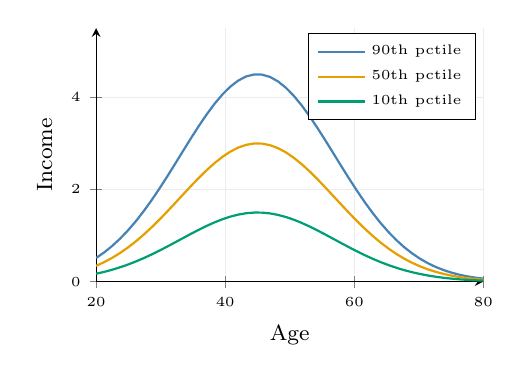
\begin{tikzpicture}
\begin{axis}[
    width=6.5cm, height=4.8cm,
    xlabel={Age}, ylabel={Income},
    xlabel style={font=\footnotesize},
    ylabel style={font=\footnotesize},
    tick label style={font=\tiny},
    xmin=20, xmax=80, ymin=0, ymax=5.5,
    grid=major, grid style={gray!15},
    legend style={font=\tiny, at={(0.98,0.98)}, anchor=north east},
    axis lines=left,
]
    \addplot[thick, softblue, domain=20:80, samples=50]
        {4.5*exp(-0.5*((x-45)/12)^2)};
    \addlegendentry{90th pctile}
    \addplot[thick, softorange, domain=20:80, samples=50]
        {3.0*exp(-0.5*((x-45)/12)^2)};
    \addlegendentry{50th pctile}
    \addplot[thick, softgreen, domain=20:80, samples=50]
        {1.5*exp(-0.5*((x-45)/12)^2)};
    \addlegendentry{10th pctile}
\end{axis}
\end{tikzpicture}\\
{\tiny Stylized income-by-age profiles}
\end{center}
\end{columns}
\end{frame}

% --- Slide 6: Dynamic Stochastic Models ---
\begin{frame}{Dynamic Stochastic General Equilibrium Models}
\textbf{Generic formulation:} find policy functions $p(\cdot)$ such that
\[
\E{G\bigl(\x_t,\,\x_{t+1},\,p(\x_t),\,p(\x_{t+1})\bigr) \;\Big|\; \x_t,\,p(\x_t)} = 0
\]
with transition law $\x_{t+1} = h\bigl(\x_t,\,p(\x_t),\,\varepsilon_{t+1}\bigr)$.

\vspace{0.4em}
\textbf{Four computational challenges} (Azinovic, Gaegauf \& Scheidegger, 2022):
\begin{enumerate}
    \setlength{\itemsep}{1pt}
    \item \emphc{Stochasticity}: nontrivial expectations over $\varepsilon_{t+1}$ and the ergodic distribution
    \item \emphc{High-dimensional} state space: heterogeneity, many assets, many shocks all push $d$ up
    \item \emphc{Strong nonlinearities / kinks} from occasionally binding constraints and regime switches
    \item \emphc{Irregular geometry} of the ergodic set: recurrent states are not a hypercube
\end{enumerate}

\vspace{0.2em}
{\footnotesize No classical method addresses all four jointly: sparse grids cover (1--3) but become impractical past $d \sim 20$ under conventional smoothness assumptions; Gaussian processes cover (1,2,4) but their $O(N^3)$ training cost limits them to small $N$.}
\end{frame}

% --- Slide 7: What is High-Dimensional? ---
\begin{frame}{What is High-Dimensional?}
\begin{center}
\begin{tabular}{rrl}
\toprule
\textbf{Dimensions $d$} & \textbf{Grid points $n^d$} & \textbf{Runtime} \\
\midrule
1 & $10$ & 10 seconds \\
2 & $100$ & 2 minutes \\
5 & $10^5$ & 1 day \\
10 & $10^{10}$ & 317 years \\
20 & $10^{20}$ & $\sim 3$ trillion years \\
\bottomrule
\end{tabular}
\end{center}

\vspace{0.5em}
{\small Assumes $n = 10$ grid points per dimension and 1 second per evaluation.}

\vspace{0.5em}
\textbf{Three remedies:}
\begin{enumerate}
    \item \emphc{Sparse grids}~(Brumm \& Scheidegger, 2017)
    \item \emphc{Random grids}~(Rust, 1997)
    \item \emphc{Neural networks}~(this lecture)
\end{enumerate}
\end{frame}

% --- Slide 8: Volumes in High Dimensions ---
\begin{frame}{Volumes in High Dimensions}
\begin{center}
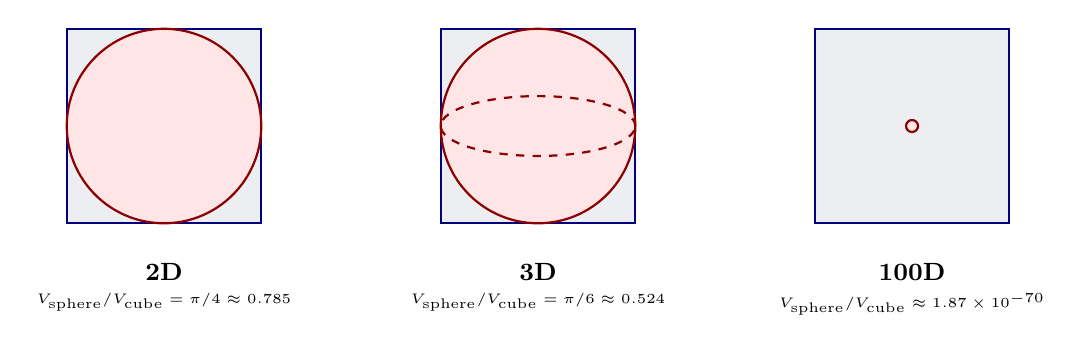
\begin{tikzpicture}[scale=0.95]
% 2D
\begin{scope}[shift={(0,0)}]
    \draw[thick, uzhblue, fill=uzhgreylight] (-1.3,-1.3) rectangle (1.3,1.3);
    \draw[thick, darkred, fill=red!10] (0,0) circle (1.3);
    \node[below, font=\small\bfseries] at (0,-1.7) {2D};
    \node[below, font=\tiny] at (0,-2.1) {$V_{\text{sphere}}/V_{\text{cube}} = \pi/4 \approx 0.785$};
\end{scope}
% 3D
\begin{scope}[shift={(5,0)}]
    \draw[thick, uzhblue, fill=uzhgreylight] (-1.3,-1.3) rectangle (1.3,1.3);
    \draw[thick, darkred, fill=red!10] (0,0) circle (1.3);
    \draw[thick, darkred, dashed] (0,0) ellipse (1.3 and 0.4);
    \node[below, font=\small\bfseries] at (0,-1.7) {3D};
    \node[below, font=\tiny] at (0,-2.1) {$V_{\text{sphere}}/V_{\text{cube}} = \pi/6 \approx 0.524$};
\end{scope}
% 100D
\begin{scope}[shift={(10,0)}]
    \draw[thick, uzhblue, fill=uzhgreylight] (-1.3,-1.3) rectangle (1.3,1.3);
    \draw[thick, darkred, fill=red!10] (0,0) circle (0.08);
    \node[below, font=\small\bfseries] at (0,-1.7) {100D};
    \node[below, font=\tiny] at (0,-2.1) {$V_{\text{sphere}}/V_{\text{cube}} \approx 1.87 \times 10^{-70}$};
\end{scope}
\end{tikzpicture}
\end{center}

\vspace{0.4em}
\begin{block}{Implication}
In high dimensions, \emphc{almost all volume is in the corners}. Grid-based methods waste most of their evaluation points in regions that barely contribute to the integral or approximation.
\end{block}
\end{frame}

% --- Slide 9: Nonlinearities and Kinks ---
\begin{frame}{Nonlinearities and Kinks}
\begin{columns}[T]
\column{0.52\textwidth}
\textbf{Where do kinks come from?}
\begin{itemize}
    \setlength{\itemsep}{1pt}
    \item \emphc{Borrowing constraints}: $a_{t+1}\ge \underline{a}$
    \item \emphc{Zero lower bound}: $i_t \ge 0$
    \item \emphc{Short-sale / participation}: corner solutions
    \item \emphc{Default, regime switches, indivisibilities}
\end{itemize}

\vspace{0.4em}
Occasionally binding constraints $\Rightarrow$ policy functions are \emphc{non-smooth} at the boundary of the binding region.

\vspace{0.4em}
{\footnotesize Polynomial / spectral methods lose accuracy; sparse grids can resolve kinks but only for $d\lesssim 20$. Neural networks handle kinks natively via ReLU-type activations.}

\column{0.48\textwidth}
\begin{center}
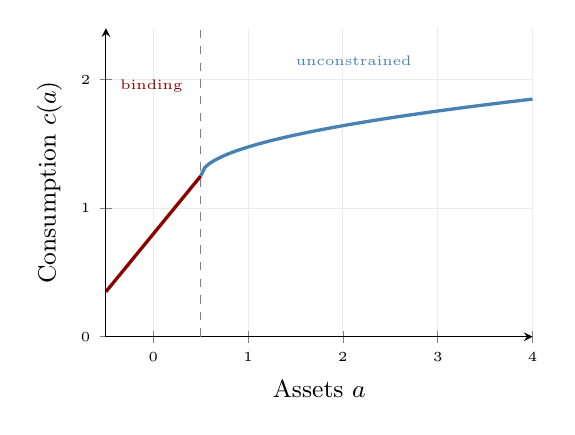
\begin{tikzpicture}
\begin{axis}[
    width=7cm, height=5.5cm,
    xlabel={Assets $a$}, ylabel={Consumption $c(a)$},
    xlabel style={font=\small},
    ylabel style={font=\small},
    tick label style={font=\tiny},
    xmin=-0.5, xmax=4, ymin=0, ymax=2.4,
    grid=major, grid style={gray!15},
    axis lines=left,
    samples=80,
]
    \addplot[very thick, darkred, domain=-0.5:0.5] {0.35 + 0.90*(x+0.5)};
    \addplot[very thick, softblue, domain=0.5:4] {1.25 + 0.32*sqrt(x-0.5)};
    \draw[dashed, gray] (axis cs:0.5,0) -- (axis cs:0.5,2.4);
    \node[font=\tiny, anchor=north] at (axis cs:0.5,0) {$a=\underline{a}$};
    \node[font=\tiny, darkred, anchor=west] at (axis cs:-0.45,1.95) {binding};
    \node[font=\tiny, softblue, anchor=west] at (axis cs:1.4,2.15) {unconstrained};
\end{axis}
\end{tikzpicture}\\
{\tiny Kinked consumption policy at the borrowing limit}
\end{center}
\end{columns}
\end{frame}

% --- Slide 10: The Ergodic Set is not a Hypercube ---
\begin{frame}{The Ergodic Set Is Not a Hypercube}
\small
\textbf{Grid-based} methods tile the full hypercube $\x \in [\x_{\min}, \x_{\max}]^d$.  \textbf{But} simulated states drawn from the model's law of motion fill only a \emphc{thin, irregular} subset, the \emphc{ergodic set} (states actually visited by the economy), often $\ll 1\%$ of the hypercube {\footnotesize (Judd, Maliar \& Maliar, 2011)}.

\vspace{0.3em}
\begin{center}
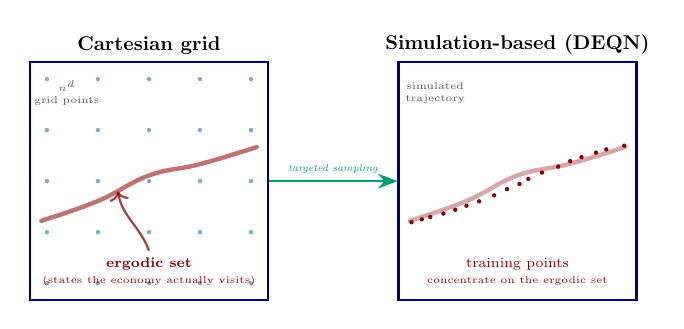
\begin{tikzpicture}[scale=0.72, transform shape,
    dotblue/.style={circle, fill=softblue!70, inner sep=0pt, minimum size=2.2pt},
    dotred/.style={circle, fill=darkred,      inner sep=0pt, minimum size=2.2pt},
    cube/.style={rectangle, draw=uzhblue, thick, minimum width=4.2cm, minimum height=4.2cm}]
    % Left panel: Cartesian grid
    \node[cube, label={above:\textbf{Cartesian grid}}] (g) at (0,0) {};
    \foreach \i in {-1.8,-0.9,0,0.9,1.8} {
        \foreach \j in {-1.8,-0.9,0,0.9,1.8} {
            \node[dotblue] at (\i,\j) {};
        }
    }
    \draw[darkred, ultra thick, opacity=0.55, line cap=round]
        plot[smooth, tension=0.7] coordinates {(-1.9,-0.7) (-0.9,-0.35) (0,0.1) (0.9,0.3) (1.9,0.6)};
    \node[font=\scriptsize, text=darkred, align=center] (ergL) at (0,-1.6)
        {\textbf{ergodic set}\\{\tiny (states the economy actually visits)}};
    \draw[->, darkred, thick, opacity=0.75]
        (ergL.north) to[out=110,in=-80,looseness=1.0] (-0.55,-0.18);
    \node[font=\tiny, text=uzhgreydark, align=center] at (-1.45,1.55) {$n^d$\\grid points};

    % Right panel: Simulation-based
    \node[cube, label={above:\textbf{Simulation-based (DEQN)}}] (s) at (6.5,0) {};
    \begin{scope}[xshift=6.5cm]
        \draw[darkred, ultra thick, opacity=0.35, line cap=round]
            plot[smooth, tension=0.7] coordinates {(-1.9,-0.7) (-0.9,-0.35) (0,0.1) (0.9,0.3) (1.9,0.6)};
        \foreach \t in {-1.85,-1.65,-1.5,-1.3,-1.1,-0.9,-0.7,-0.45,-0.2,0,0.2,0.45,0.7,0.95,1.15,1.4,1.6,1.85}{
            \pgfmathsetmacro{\yy}{-0.7 + 1.3*(\t + 1.9)/3.8 + 0.08*sin(deg(\t*1.4))}
            \pgfmathsetmacro{\xx}{\t + 0.04*rand}
            \node[dotred] at (\xx,\yy) {};
        }
        \node[font=\tiny, text=uzhgreydark, align=center] at (-1.45,1.55)
            {simulated\\trajectory};
        \node[font=\scriptsize, text=darkred, align=center] at (0,-1.6)
            {training points\\{\tiny concentrate on the ergodic set}};
    \end{scope}

    \draw[-{Stealth[length=2.5mm]}, thick, softgreen]
        (g.east) -- node[above, font=\tiny, text=softgreen]{\textit{targeted sampling}} (s.west);
\end{tikzpicture}
\end{center}

\vspace{-0.3em}
\begin{center}
{\footnotesize A full Cartesian grid \emphc{wastes} most of its work in regions the economy never visits $\Rightarrow$ motivates \emphc{simulation-based, grid-free} methods.}
\end{center}
\end{frame}

% --- Slide 11: Abstract Problem Formulation ---
\begin{frame}{Abstract Problem Formulation}
We need a numerical method that satisfies:

\vspace{0.4em}
\begin{enumerate}
    \item \textbf{Global approximation:} avoid purely local perturbation solutions
    \item \textbf{Approximate solutions:} accept small residual error $\varepsilon > 0$
    \item \textbf{Grid-free in practice:} avoid explicit tensor-product growth $n^d$
    \item \textbf{Flexible geometry:} handle nonlinearities, kinks, and irregular ergodic sets
    \item \textbf{Parallel-friendly:} benefit from \emphc{parallelization} on modern hardware
\end{enumerate}

\vspace{0.6em}
\begin{center}
$\Rightarrow$ \textbf{DEQNs address this wishlist well in practice,}
while \emphc{mitigating} rather than eliminating high-dimensional costs.
\end{center}
\end{frame}

% --- Slide 10: Our Solution: DEQNs ---
\begin{frame}{Our Solution: Deep Equilibrium Nets}
\textbf{Core idea} (Azinovic, Gaegauf \& Scheidegger, 2022):

\vspace{0.3em}
Replace the traditional grid-based solution with a \emphc{neural network} trained to satisfy economic equilibrium conditions.

\vspace{0.5em}
\begin{block}{Three Key Ingredients}
\begin{enumerate}
    \item \textbf{Equilibrium error as loss function:} use the economic equations $G(\cdot) = 0$ directly, with \emphc{no labeled data} needed
    \item \textbf{Stochastic gradient descent:} optimize network parameters $\rho$ via SGD on mini-batches
    \item \textbf{Simulated paths:} draw training points from the \emphc{ergodic distribution} of the model itself
\end{enumerate}
\end{block}

\vspace{0.3em}
{\small $\Rightarrow$ This turns \emphc{solving} an economic model into \emphc{training} a neural network.}
\\[2pt]
{\scriptsize It avoids explicit state-space grids, but expectation accuracy, sampling quality, and optimization still matter.}
\end{frame}

% ============================================================================
% PART II: FROM ANNs TO DEQNs
% ============================================================================

% --- Slide 11: Section Divider ---
\begin{frame}{}
\vfill
\begin{center}
{\Huge \textcolor{uzhblue}{\textbf{Part II}}}\\[12pt]
{\LARGE From ANNs to Deep Equilibrium Nets}
\end{center}
\vfill
\end{frame}

% --- Slide 12: What is a DNN? ---
\begin{frame}{What is a Deep Neural Network?}
A deep neural network (DNN) $\mathcal{N}_\rho : \R^{d_{\text{in}}} \to \R^{d_{\text{out}}}$ is a \emphc{parametric function approximator}.

\vspace{0.5em}
\textbf{Universal approximation} (Cybenko 1989, Hornik et al.\ 1989):
\[
\forall f \in C(\mathcal{K},\R),\ \forall\varepsilon > 0,\;\; \exists\, \rho^\star : \quad \sup_{\x\in\mathcal{K}}\bigl\|\mathcal{N}_{\rho^\star}(\x) - f(\x)\bigr\| < \varepsilon
\]
{\scriptsize ($\mathcal{K}\subset\R^{d_{\mathrm{in}}}$ compact; the norm is the supremum over $\mathcal{K}$.)}

\vspace{0.5em}
\textbf{In economics:}
\begin{itemize}
    \item \emphc{Input:} state variables $\x_t \in \R^{d}$ (capital, productivity, wealth distribution, \ldots)
    \item \emphc{Output:} policy variables (consumption, savings, prices, \ldots)
    \item \emphc{Parameters} $\rho$: weights and biases, found by \emphc{training}
\end{itemize}
\end{frame}

% --- Slide 13: DNN Layer Structure ---
\begin{frame}{DNN Layer Structure}
\begin{center}
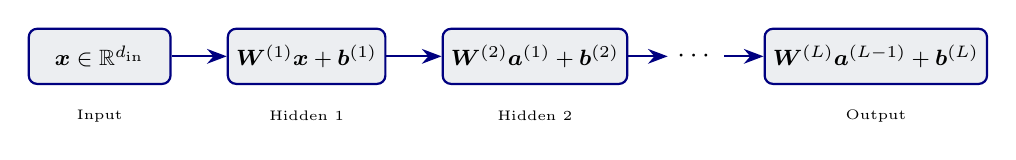
\begin{tikzpicture}[
    mlstep/.style={rectangle, draw=uzhblue, thick, fill=uzhgreylight,
        minimum width=1.8cm, minimum height=0.7cm, font=\footnotesize,
        rounded corners=3pt, inner sep=3pt},
    arr/.style={-{Stealth[length=2.5mm]}, thick, uzhblue}
]
    \node[mlstep] (in) {$\x \in \R^{d_{\text{in}}}$};
    \node[mlstep, right=0.7cm of in] (h1) {$\W^{(1)}\x + \bb^{(1)}$};
    \node[mlstep, right=0.7cm of h1] (h2) {$\W^{(2)}\a^{(1)} + \bb^{(2)}$};
    \node[right=0.5cm of h2, font=\normalsize] (dots) {$\cdots$};
    \node[mlstep, right=0.5cm of dots] (out) {$\W^{(L)}\a^{(L-1)} + \bb^{(L)}$};

    \draw[arr] (in) -- (h1);
    \draw[arr] (h1) -- (h2);
    \draw[arr] (h2) -- (dots);
    \draw[arr] (dots) -- (out);

    \node[below=0.2cm, font=\tiny] at (in.south) {Input};
    \node[below=0.2cm, font=\tiny] at (h1.south) {Hidden 1};
    \node[below=0.2cm, font=\tiny] at (h2.south) {Hidden 2};
    \node[below=0.2cm, font=\tiny] at (out.south) {Output};
\end{tikzpicture}
\end{center}

\vspace{0.4em}
Each layer performs an \emphc{affine transformation}:
\[
\z^{(\ell)} = \W^{(\ell)} \a^{(\ell-1)} + \bb^{(\ell)}, \qquad \ell = 1, \ldots, L
\]
where $\W^{(\ell)} \in \R^{n_\ell \times n_{\ell-1}}$ and $\bb^{(\ell)} \in \R^{n_\ell}$.

\vspace{0.3em}
{\small Without nonlinear activations, the entire network collapses to a single affine map.}
\end{frame}

% --- Slide 14: Activation Functions ---
\begin{frame}{Activation Functions}
\begin{center}
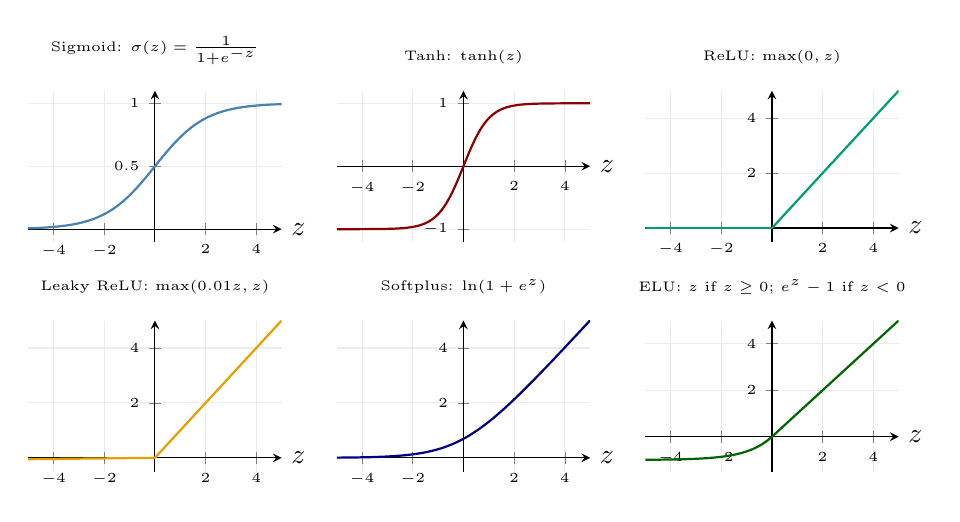
\begin{tikzpicture}
% Row 1: Sigmoid, Tanh, ReLU
\begin{axis}[
    name=plot1,
    width=4.8cm, height=3.5cm,
    title={\tiny Sigmoid: $\sigma(z) = \frac{1}{1+e^{-z}}$},
    title style={font=\tiny},
    xlabel={$z$}, xlabel style={font=\tiny},
    tick label style={font=\tiny},
    xmin=-5, xmax=5, ymin=-0.1, ymax=1.1,
    grid=major, grid style={gray!15},
    axis lines=middle,
    every axis x label/.style={at={(current axis.right of origin)}, anchor=west},
]
    \addplot[thick, softblue, domain=-5:5, samples=100]{1/(1+exp(-x))};
\end{axis}

\begin{axis}[
    at={($(plot1.east)+(0.7cm,0)$)}, anchor=west,
    name=plot2,
    width=4.8cm, height=3.5cm,
    title={\tiny Tanh: $\tanh(z)$},
    title style={font=\tiny},
    xlabel={$z$}, xlabel style={font=\tiny},
    tick label style={font=\tiny},
    xmin=-5, xmax=5, ymin=-1.2, ymax=1.2,
    grid=major, grid style={gray!15},
    axis lines=middle,
    every axis x label/.style={at={(current axis.right of origin)}, anchor=west},
]
    \addplot[thick, darkred, domain=-5:5, samples=100]{tanh(x)};
\end{axis}

\begin{axis}[
    at={($(plot2.east)+(0.7cm,0)$)}, anchor=west,
    name=plot3,
    width=4.8cm, height=3.5cm,
    title={\tiny ReLU: $\max(0,z)$},
    title style={font=\tiny},
    xlabel={$z$}, xlabel style={font=\tiny},
    tick label style={font=\tiny},
    xmin=-5, xmax=5, ymin=-0.5, ymax=5,
    grid=major, grid style={gray!15},
    axis lines=middle,
    every axis x label/.style={at={(current axis.right of origin)}, anchor=west},
]
    \addplot[thick, softgreen, domain=-5:0, samples=2]{0};
    \addplot[thick, softgreen, domain=0:5, samples=2]{x};
\end{axis}

% Row 2: Leaky ReLU, Softplus, ELU
\begin{axis}[
    at={($(plot1.south)-(0,1.0cm)$)}, anchor=north,
    name=plot4,
    width=4.8cm, height=3.5cm,
    title={\tiny Leaky ReLU: $\max(0.01z,z)$},
    title style={font=\tiny},
    xlabel={$z$}, xlabel style={font=\tiny},
    tick label style={font=\tiny},
    xmin=-5, xmax=5, ymin=-0.5, ymax=5,
    grid=major, grid style={gray!15},
    axis lines=middle,
    every axis x label/.style={at={(current axis.right of origin)}, anchor=west},
]
    \addplot[thick, softorange, domain=-5:0, samples=2]{0.01*x};
    \addplot[thick, softorange, domain=0:5, samples=2]{x};
\end{axis}

\begin{axis}[
    at={($(plot2.south)-(0,1.0cm)$)}, anchor=north,
    name=plot5,
    width=4.8cm, height=3.5cm,
    title={\tiny Softplus: $\ln(1+e^z)$},
    title style={font=\tiny},
    xlabel={$z$}, xlabel style={font=\tiny},
    tick label style={font=\tiny},
    xmin=-5, xmax=5, ymin=-0.5, ymax=5,
    grid=major, grid style={gray!15},
    axis lines=middle,
    every axis x label/.style={at={(current axis.right of origin)}, anchor=west},
]
    \addplot[thick, uzhblue, domain=-5:5, samples=100]{ln(1+exp(x))};
\end{axis}

\begin{axis}[
    at={($(plot3.south)-(0,1.0cm)$)}, anchor=north,
    name=plot6,
    width=4.8cm, height=3.5cm,
    title={\tiny ELU: $z$ if $z\ge 0$; $e^z-1$ if $z<0$},
    title style={font=\tiny},
    xlabel={$z$}, xlabel style={font=\tiny},
    tick label style={font=\tiny},
    xmin=-5, xmax=5, ymin=-1.5, ymax=5,
    grid=major, grid style={gray!15},
    axis lines=middle,
    every axis x label/.style={at={(current axis.right of origin)}, anchor=west},
]
    \addplot[thick, darkgreen, domain=-5:0, samples=100]{exp(x)-1};
    \addplot[thick, darkgreen, domain=0:5, samples=2]{x};
\end{axis}
\end{tikzpicture}
\end{center}
\end{frame}

% --- Slide 15: DNN with Activations ---
\begin{frame}{DNN with Nonlinear Activations}
\begin{center}
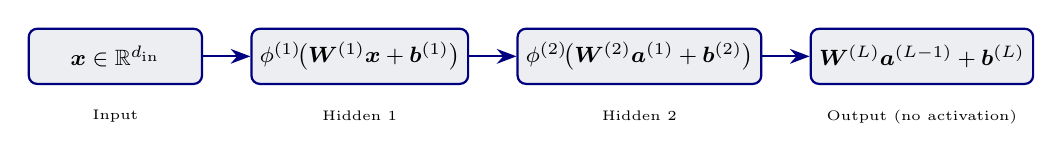
\begin{tikzpicture}[
    mlstep/.style={rectangle, draw=uzhblue, thick, fill=uzhgreylight,
        minimum width=2.2cm, minimum height=0.7cm, font=\footnotesize,
        rounded corners=3pt, inner sep=3pt},
    arr/.style={-{Stealth[length=2.5mm]}, thick, uzhblue}
]
    \node[mlstep] (in) {$\x \in \R^{d_{\text{in}}}$};
    \node[mlstep, right=0.6cm of in] (h1) {$\phi^{(1)}\!\bigl(\W^{(1)}\x + \bb^{(1)}\bigr)$};
    \node[mlstep, right=0.6cm of h1] (h2) {$\phi^{(2)}\!\bigl(\W^{(2)}\a^{(1)} + \bb^{(2)}\bigr)$};
    \node[mlstep, right=0.6cm of h2] (out) {$\W^{(L)}\a^{(L-1)} + \bb^{(L)}$};

    \draw[arr] (in) -- (h1);
    \draw[arr] (h1) -- (h2);
    \draw[arr] (h2) -- (out);

    \node[below=0.2cm, font=\tiny] at (in.south) {Input};
    \node[below=0.2cm, font=\tiny] at (h1.south) {Hidden 1};
    \node[below=0.2cm, font=\tiny] at (h2.south) {Hidden 2};
    \node[below=0.2cm, font=\tiny] at (out.south) {Output (no activation)};
\end{tikzpicture}
\end{center}

\vspace{0.3em}
Each hidden layer applies a \emphc{nonlinear activation} $\phi^{(\ell)}$:
\[
\a^{(\ell)} = \phi^{(\ell)}\!\bigl(\W^{(\ell)} \a^{(\ell-1)} + \bb^{(\ell)}\bigr), \qquad \ell = 1, \ldots, L-1
\]

\vspace{0.2em}
\begin{itemize}
    \item The output layer is typically \emphc{linear} (for regression) or uses \emphc{softplus} (to enforce positivity, e.g.\ consumption)
    \item The full network: $\mathcal{N}_\rho(\x) = \W^{(L)} \a^{(L-1)} + \bb^{(L)}$
\end{itemize}
\end{frame}

% --- Slide 16: Finding Parameters (Supervised) ---
\begin{frame}{Finding Parameters: Supervised Learning}
\textbf{Standard approach} (when labeled data $\{(\x_i, y_i)\}_{i=1}^N$ are available):

\vspace{0.5em}
\begin{enumerate}
    \item \textbf{Collect labeled data:}~~$\x_i \xrightarrow{\text{true mapping}} y_i$

    \vspace{0.3em}
    \item \textbf{Define a loss function:}
    \[
    \ell_\rho^{\text{sup}} = \frac{1}{N}\sum_{i=1}^{N} \bigl\|y_i - \mathcal{N}_\rho(\x_i)\bigr\|^2
    \qquad\text{(mean squared error)}
    \]

    \vspace{0.3em}
    \item \textbf{Update via SGD} ($\eta$ = learning rate; the symbol $\alpha$ is reserved for the Cobb--Douglas capital share later in the deck):
    \[
    \rho^{\text{new}} = \rho^{\text{old}} - \eta \cdot \frac{\partial \ell_\rho}{\partial \rho}\bigg|_{\rho = \rho^{\text{old}}}
    \]
\end{enumerate}

\vspace{0.3em}
{\small This is the recipe from Lecture~1. But in economics, \emphc{we rarely have labeled data}\ldots}
\end{frame}

% --- Slide 17: The Data Problem ---
\begin{frame}{The ``Data Problem'' in Economics}
\textbf{Deep learning excels} when massive labeled datasets are available.

\vspace{0.5em}
\textbf{But in computational economics:}
\begin{itemize}
    \item We solve \emphc{functional equations}, not classification/regression tasks
    \item There are \emphc{no labeled pairs} $(\x_i, y_i)$
    \item Traditional approach: \emphc{time iteration on a grid}, but grids do not scale
\end{itemize}

\vspace{0.5em}
\textbf{Key insight:}
\begin{itemize}
    \item We \emphc{know} the structural equations $G(\cdot) = 0$
    \item We can \emphc{check} how well a candidate policy satisfies them
    \item $\Rightarrow$ Use the \emphc{equilibrium error} as the loss function!
\end{itemize}
\end{frame}

% --- Slide 18: Issue with Time Iteration ---
\begin{frame}{Traditional Approach: Time Iteration on a Grid}
\begin{alertblock}{Algorithm: Grid-Based Collocation}
\begin{algorithmic}
\small
\STATE \textbf{Input:} Grid $\mathcal{G} = \{\x_1, \ldots, \x_M\} \subset \R^d$, initial guess $p^{(0)}$
\FOR{$k = 0, 1, 2, \ldots$ until convergence}
    \FOR{each grid point $\x_i \in \mathcal{G}$}
        \STATE Solve $G\bigl(\x_i,\, p^{(k)}(\x_i),\, p^{(k)}\bigr) = 0$ for $p^{(k+1)}(\x_i)$
    \ENDFOR
    \STATE Interpolate $p^{(k+1)}$ between grid points
\ENDFOR
\end{algorithmic}
\end{alertblock}

\vspace{0.3em}
\textbf{Problems:}
\begin{itemize}
    \item \emphc{Cartesian} grids need $M=n^d$ points, infeasible beyond $d\sim4\text{--}5$ at sensible resolution ($10^5$ at $d\!=\!5$, $10^{10}$ at $d\!=\!10$)
    \item \emphc{Sparse grids} (Smolyak, adaptive) extend the practical reach only to $d \sim 20\text{--}50$
    \item Heterogeneous-agent or many-country DSGE models routinely need $d \gg 50$, beyond any grid-based method
\end{itemize}
\end{frame}

% --- Slide 19: Economic Loss Function ---
\begin{frame}{The DEQN Loss Function}
\textbf{Key idea:} replace labeled data with \emphc{economic equilibrium conditions}.

\vspace{0.5em}
Let $G(\x, f(\x)) = 0$ be the system of equilibrium equations. Define:
\[
\boxed{
\ell_\rho = \frac{1}{N} \sum_{i=1}^{N} \bigl\| G\bigl(\x_i,\, \mathcal{N}_\rho(\x_i)\bigr) \bigr\|^2
}
\]

\vspace{0.3em}
\begin{itemize}
    \item $\mathcal{N}_\rho(\x_i)$ is the neural net's \emphc{predicted policy} at state $\x_i$
    \item $G(\cdot)$ measures the \emphc{equilibrium error} (e.g.\ Euler equation residual)
    \item Small $\ell_\rho$ means the policy nearly satisfies the equations on the sampled states
\end{itemize}

\vspace{0.5em}
$\Rightarrow$ \emphc{No labels needed}; we call this \textbf{self-supervised} learning (sometimes labelled ``unsupervised'' in the narrow no-labels sense).
\\[2pt]
{\scriptsize In stochastic models, expectations inside $G$ are approximated, e.g.\ by path averaging or quadrature.}
\end{frame}

% --- Slide 20: Inside one DEQN step ---
\begin{frame}{Inside One DEQN Training Step}
\begin{center}
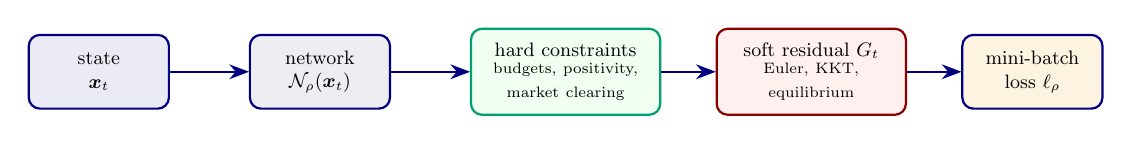
\begin{tikzpicture}[scale=0.78, transform shape,
    box/.style={rectangle, draw=uzhblue, thick, rounded corners=4pt,
                text width=2.0cm, minimum height=1.2cm, align=center, font=\small, inner sep=4pt},
    hard/.style={rectangle, draw=softgreen, thick, rounded corners=4pt,
                fill=green!6, text width=2.8cm, minimum height=1.4cm, align=center, font=\small, inner sep=4pt},
    soft/.style={rectangle, draw=darkred, thick, rounded corners=4pt,
                fill=red!6, text width=2.8cm, minimum height=1.4cm, align=center, font=\small, inner sep=4pt},
    arr/.style={-{Stealth[length=2.5mm]}, thick, uzhblue}
]
    \node[box, fill=uzhblue!8]    (x)    at ( 0.0, 0) {state\\$\x_t$};
    \node[box, fill=uzhgreylight] (nn)   at ( 3.6, 0) {network\\$\mathcal{N}_\rho(\x_t)$};
    \node[hard]                   (hc)   at ( 7.6, 0) {hard constraints\\\scriptsize budgets, positivity,\\\scriptsize market clearing};
    \node[soft]                   (res)  at (11.6, 0) {soft residual $G_t$\\\scriptsize Euler, KKT,\\\scriptsize equilibrium};
    \node[box, fill=softorange!12](loss) at (15.2, 0) {mini-batch\\loss $\ell_\rho$};

    \draw[arr] (x)   -- (nn);
    \draw[arr] (nn)  -- (hc);
    \draw[arr] (hc)  -- (res);
    \draw[arr] (res) -- (loss);
\end{tikzpicture}
\end{center}

\vspace{0.4em}
\begin{itemize}
    \item Encode what can be enforced \emphc{exactly} in the architecture.
    \item Minimize only the genuinely non-closed-form equilibrium conditions.
    \item Draw states from the model's own simulation, so training focuses on the ergodic set.
\end{itemize}
\end{frame}

% --- Slide 21: Training DEQN Algorithm ---
\begin{frame}{Training Algorithm for DEQNs}
\begin{block}{Algorithm 1: Deep Equilibrium Net Training}
\begin{algorithmic}
\footnotesize
\STATE \textbf{Input:} Initial state $\x_0$, network $\mathcal{N}_\rho$, learning rate $\eta$, episodes $E$, simulation horizon $T_{\mathrm{sim}}$, training steps $T_{\mathrm{train}}$
\FOR{episode $e = 1, \ldots, E$}
    \STATE \textbf{Simulate path:} $\x_0 \to \x_1 \to \cdots \to \x_{T_{\mathrm{sim}}}$ using $\mathcal{N}_\rho$ and transition law
    \FOR{gradient step $t = 1, \ldots, T_{\mathrm{train}}$}
        \STATE Draw mini-batch $\mathcal{B} \subset \{\x_0, \ldots, \x_{T_{\mathrm{sim}}}\}$
        \STATE Compute loss:~$\ell_\rho = \frac{1}{|\mathcal{B}|}\sum_{\x_i \in \mathcal{B}} \|G(\x_i, \mathcal{N}_\rho(\x_i))\|^2$
        \STATE Update:~$\rho \leftarrow \rho - \eta \cdot \nabla_\rho \ell_\rho$
    \ENDFOR
\ENDFOR
\STATE \textbf{Output:} Trained network $\mathcal{N}_{\rho^\star}$ approximating the policy function
\end{algorithmic}
\end{block}

\vspace{0.2em}
{\small \textbf{Note:} Training points come from the \emphc{model's own simulation}, so the network learns on the ergodic distribution, focusing on economically relevant regions.}
\end{frame}

% --- Slide 21: Supervised vs Self-Supervised ---
\begin{frame}{Supervised vs.\ Self-Supervised (DEQN) Learning}
\begin{columns}[T]
\column{0.47\textwidth}
\begin{center}
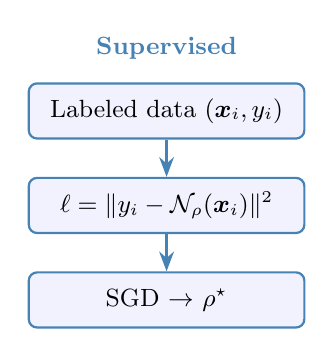
\begin{tikzpicture}[
    mlstep/.style={rectangle, draw=softblue, thick, fill=blue!5,
        minimum width=3.5cm, minimum height=0.7cm, font=\small,
        rounded corners=3pt},
    arr/.style={-{Stealth[length=2.5mm]}, thick, softblue}
]
    \node[font=\small\bfseries, softblue] at (0,3.2) {Supervised};
    \node[mlstep] (d) at (0,2.4) {Labeled data $(\x_i, y_i)$};
    \node[mlstep] (l) at (0,1.2) {$\ell = \|y_i - \mathcal{N}_\rho(\x_i)\|^2$};
    \node[mlstep] (s) at (0,0) {SGD $\to$ $\rho^\star$};
    \draw[arr] (d) -- (l);
    \draw[arr] (l) -- (s);
\end{tikzpicture}
\end{center}

\column{0.47\textwidth}
\begin{center}
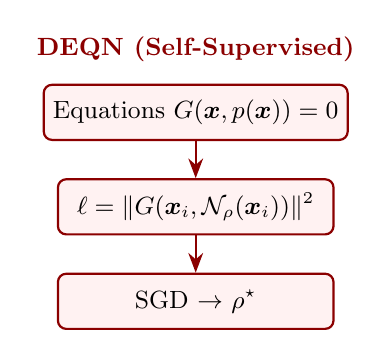
\begin{tikzpicture}[
    mlstep/.style={rectangle, draw=darkred, thick, fill=red!5,
        minimum width=3.5cm, minimum height=0.7cm, font=\small,
        rounded corners=3pt},
    arr/.style={-{Stealth[length=2.5mm]}, thick, darkred}
]
    \node[font=\small\bfseries, darkred] at (0,3.2) {DEQN (Self-Supervised)};
    \node[mlstep] (d) at (0,2.4) {Equations $G(\x, p(\x))=0$};
    \node[mlstep] (l) at (0,1.2) {$\ell = \|G(\x_i, \mathcal{N}_\rho(\x_i))\|^2$};
    \node[mlstep] (s) at (0,0) {SGD $\to$ $\rho^\star$};
    \draw[arr] (d) -- (l);
    \draw[arr] (l) -- (s);
\end{tikzpicture}
\end{center}
\end{columns}

\vspace{0.5em}
\begin{center}
{\small \emphc{Key difference:} DEQNs replace labeled data with structural economic equations.}
\end{center}
\end{frame}

% --- Slide 22: DEQN Key Recap ---
\begin{frame}{DEQN: Key Recap}
\begin{columns}[T]
\column{0.32\textwidth}
\begin{block}{Replace Labels}
\centering
\small
Instead of labeled data $(\x_i, y_i)$, use the economic equilibrium equations $G(\cdot) = 0$ as the loss.
\end{block}

\column{0.32\textwidth}
\begin{block}{Replace Grids}
\centering
\small
Instead of $n^d$ grid points, use a neural network $\mathcal{N}_\rho$ that maps states to policies \emphc{globally}.
\end{block}

\column{0.32\textwidth}
\begin{block}{Replace TI}
\centering
\small
Instead of time iteration with interpolation, use SGD on simulated paths from the model.
\end{block}
\end{columns}

\vspace{0.8em}
\begin{center}
\textbf{Result:} A grid-free, simulation-based method that can handle
much higher-dimensional models than standard grids and maps naturally to GPUs.
\end{center}
\end{frame}

% ============================================================================
% PART III: BROCK--MIRMAN BENCHMARK
% ============================================================================

% --- Slide 23: Section Divider ---
\begin{frame}{}
\vfill
\begin{center}
{\Huge \textcolor{uzhblue}{\textbf{Part III}}}\\[12pt]
{\LARGE Brock--Mirman Benchmark}
\end{center}
\vfill
\end{frame}

% --- Slide 24: Brock-Mirman Setup ---
\begin{frame}{Brock--Mirman (1972): Setup}
\footnotesize
\textbf{Social planner's problem.} Choose a consumption sequence to maximize expected lifetime log utility:
\[
\max_{\{C_t\}_{t=0}^{\infty}} \; \E{\sum_{t=0}^{\infty} \beta^t \ln C_t}
\]

\vspace{0.2em}
\textbf{Resource constraint} (full depreciation, $\delta = 1$):
\[
C_t + K_{t+1} \;=\; z_t K_t^{\alpha}, \qquad K_0 > 0 \text{ given.}
\]

\vspace{0.2em}
\textbf{Stochastic productivity.} TFP $z_t$ follows an AR(1) in logs:
\[
\ln z_{t+1} \;=\; \varrho \ln z_t + \sigma_z\, \epsilon_{t+1}, \qquad \epsilon_{t+1} \sim \mathcal{N}(0,1).
\]

\vspace{0.2em}
\textbf{State \& control.} State $\bm{x}_t = (K_t, z_t)$; control $C_t$. Capital then follows from the budget as $K_{t+1} = z_t K_t^\alpha - C_t$.

\vspace{0.4em}
{\footnotesize\emphc{Next two slides:} derive the Euler equation from first principles, then obtain the closed-form policy -- the benchmark we will later compare the DEQN solution to.}
\end{frame}

% --- Slide 25: Deriving the Euler equation (Lagrangian) ---
\begin{frame}{Deriving the Euler Equation (Lagrangian)}
\footnotesize
\textbf{Step 1. Lagrangian.} Attach a multiplier $\lambda_t \ge 0$ to each period's budget constraint:
\[
\mathcal{L} \;=\; \E{\sum_{t=0}^{\infty} \beta^t \Big[\, \ln C_t \;-\; \lambda_t\,\big( C_t + K_{t+1} - z_t K_t^{\alpha} \big) \Big]}.
\]

\vspace{0.2em}
\textbf{Step 2. Take partial derivatives} with respect to the choices at date $t$:
\begin{columns}[T]
\column{0.48\textwidth}
\emphc{Consumption FOC} $\;\partial\mathcal{L}/\partial C_t = 0$:
\[
\beta^t\!\left( \frac{1}{C_t} - \lambda_t \right) = 0
\;\;\Longrightarrow\;\; \lambda_t = \frac{1}{C_t}.
\]

\column{0.52\textwidth}
\emphc{Capital FOC} $\;\partial\mathcal{L}/\partial K_{t+1} = 0$:
\[
-\beta^t \lambda_t \;+\; \beta^{t+1}\,\E{\lambda_{t+1}\,\alpha z_{t+1} K_{t+1}^{\alpha-1}} = 0.
\]
\end{columns}

\vspace{0.3em}
\textbf{Step 3. Eliminate $\lambda$.} Substitute $\lambda_t = 1/C_t$, $\lambda_{t+1} = 1/C_{t+1}$ and divide by $\beta^t$:
\[
\boxed{\;\; \frac{1}{C_t} \;=\; \beta\, \E{\frac{\alpha\, z_{t+1}\, K_{t+1}^{\alpha-1}}{C_{t+1}}} \;\;} \quad \text{(stochastic Euler equation)}
\]

\vspace{0.2em}
{\scriptsize\emphc{Reading:} marginal utility of today's consumption $\; = \;$ discounted expected marginal utility of tomorrow's consumption $\,\times\,$ gross marginal product of capital at $t{+}1$. The transversality condition $\lim_{t\to\infty}\E{\beta^t \lambda_t K_{t+1}} = 0$ rules out bubbles.}
\end{frame}

% --- Slide 26: Closed-form policy (guess-and-verify) ---
\begin{frame}{Closed-Form Policy via Guess-and-Verify}
\footnotesize
\textbf{Guess.} Consumption is a constant fraction $1-\phi$ of output:
\[
C_t \;=\; (1-\phi)\, z_t K_t^{\alpha}, \qquad \phi \in (0,1)\ \text{to be determined.}
\]
The budget then implies $K_{t+1} = \phi\, z_t K_t^{\alpha}$.

\vspace{0.2em}
\textbf{Substitute into the Euler equation.} With $C_{t+1} = (1-\phi)\, z_{t+1} K_{t+1}^{\alpha}$,
\[
\frac{\alpha\, z_{t+1}\, K_{t+1}^{\alpha-1}}{C_{t+1}}
\;=\; \frac{\alpha\, z_{t+1}\, K_{t+1}^{\alpha-1}}{(1-\phi)\, z_{t+1}\, K_{t+1}^{\alpha}}
\;=\; \frac{\alpha}{(1-\phi)\, K_{t+1}}.
\]
\emphc{Note:} $z_{t+1}$ cancels, so the conditional expectation collapses (log $+$ Cobb--Douglas $+$ full depreciation).

\vspace{0.2em}
\textbf{Solve for $\phi$.} Plug $K_{t+1} = \phi z_t K_t^\alpha$ on both sides of the Euler:
\[
\underbrace{\frac{1}{(1-\phi)\, z_t K_t^{\alpha}}}_{\text{LHS}}
\;=\; \beta\, \cdot\, \underbrace{\frac{\alpha}{(1-\phi)\, \phi\, z_t K_t^{\alpha}}}_{\text{RHS}}
\;\;\Longrightarrow\;\; 1 = \frac{\beta\alpha}{\phi}
\;\;\Longrightarrow\;\; \phi = \beta\alpha.
\]

\vspace{0.2em}
\textbf{Closed-form policy.}
\[
\boxed{\;\; C_t \;=\; (1-\beta\alpha)\, z_t K_t^{\alpha},
\qquad K_{t+1} \;=\; \beta\alpha\, z_t K_t^{\alpha} \;\;}
\]

{\scriptsize This benchmark provides an analytic target against which we will measure the DEQN's trained policy.}
\end{frame}

% --- Slide 27: Brock-Mirman hard/soft split ---
\begin{frame}[shrink=10]{Brock--Mirman: Hard vs.\ Soft Constraints}
\small
\textbf{Split the equilibrium conditions by what the architecture can enforce exactly.}

\vspace{0.2em}
\begin{center}
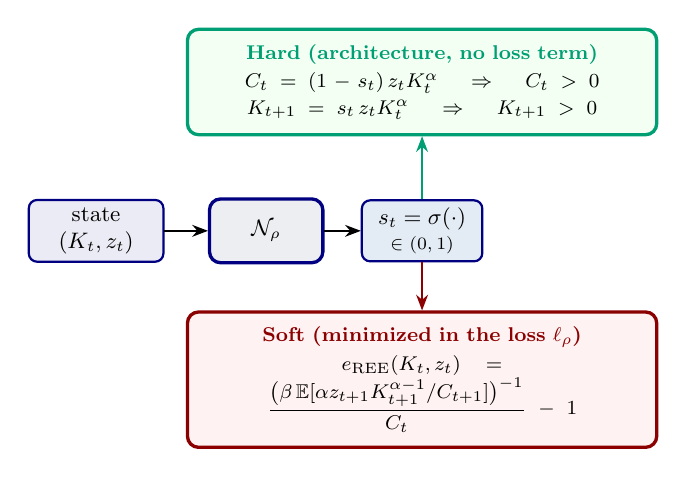
\begin{tikzpicture}[scale=0.90, transform shape,
    io/.style={rectangle, draw=uzhblue, thick, rounded corners=3pt, fill=uzhblue!8,
               minimum width=1.9cm, minimum height=0.8cm, font=\small, align=center, inner sep=3pt},
    dnn/.style={rectangle, draw=uzhblue, very thick, rounded corners=4pt, fill=uzhgreylight,
               minimum width=1.6cm, minimum height=0.9cm, font=\small\bfseries, align=center},
    sig/.style={rectangle, draw=uzhblue, thick, rounded corners=3pt, fill=softblue!15,
               minimum width=1.7cm, minimum height=0.8cm, font=\small, align=center, inner sep=3pt},
    hard/.style={rectangle, draw=softgreen, very thick, rounded corners=4pt, fill=green!5,
               text width=6.2cm, font=\footnotesize, align=center, inner sep=6pt},
    soft/.style={rectangle, draw=darkred, very thick, rounded corners=4pt, fill=red!5,
               text width=6.2cm, font=\footnotesize, align=center, inner sep=6pt},
    arr/.style={-{Stealth[length=2mm]}, thick}
]
    % Center spine: state -> N_rho -> sigmoid(s_t)
    \node[io]  (x)  at (0,0) {state\\$(K_t,z_t)$};
    \node[dnn] (nn) at (2.4,0) {$\mathcal{N}_\rho$};
    \node[sig] (s)  at (4.6,0) {$s_t=\sigma(\cdot)$\\[-1pt]{\scriptsize $\in(0,1)$}};
    \draw[arr] (x)  -- (nn);
    \draw[arr] (nn) -- (s);

    % Hard constraints (top, green)
    \node[hard] (H) at (4.6, 2.1)
        {\textbf{\textcolor{softgreen}{Hard (architecture, no loss term)}}\\[2pt]
         $C_t = (1-s_t)\,z_tK_t^\alpha \quad\Rightarrow\quad C_t>0$ \\[1pt]
         $K_{t+1} = s_t\,z_tK_t^\alpha \quad\Rightarrow\quad K_{t+1}>0$};
    \draw[arr, softgreen, thick] (s.north) -- (H.south);

    % Soft residual (bottom, red)
    \node[soft] (S) at (4.6,-2.1)
        {\textbf{\textcolor{darkred}{Soft (minimized in the loss $\ell_\rho$)}}\\[2pt]
         $e_{\mathrm{REE}}(K_t,z_t) = \dfrac{\bigl(\beta\,\mathbb{E}[\alpha z_{t+1}K_{t+1}^{\alpha-1}/C_{t+1}]\bigr)^{-1}}{C_t}\,-\,1$};
    \draw[arr, darkred, thick] (s.south) -- (S.north);
\end{tikzpicture}
\end{center}

\vspace{-0.25em}
{\footnotesize
\emphc{Why bother?} A softplus head on $C_t$ alone would secure $C_t\!>\!0$ but could push $K_{t+1}\!<\!0$.  The sigmoid-savings head removes \emph{both} failure modes before training starts.  Only the genuinely non-closed-form condition, the Euler equation, enters the loss.}
\end{frame}

% --- Slide 28: Brock-Mirman residual ---
\begin{frame}[shrink=10]{Brock--Mirman: Residual, Expectation, Loss}
\textbf{Pathwise residual used in the notebook} (full-depreciation $\delta=1$ benchmark):
\[
G_t = 1 - \beta \, \frac{C_t}{C_{t+1}} \cdot \alpha z_{t+1} K_{t+1}^{\alpha-1},
\]
with
\[
K_{t+1} = s_t z_t K_t^\alpha, \qquad
C_{t+1} = (1-s_{t+1}) z_{t+1} K_{t+1}^\alpha.
\]

\vspace{-0.2em}
{\scriptsize\emphc{Partial depreciation.}  The uncertainty notebook uses $\delta=0.1$; the marginal productivity of capital then becomes $\alpha z_{t+1} K_{t+1}^{\alpha-1} + (1-\delta)$ and $K_{t+2} = z_{t+1} K_{t+1}^{\alpha} + (1-\delta) K_{t+1} - C_{t+1}$.  The closed-form $\phi = \alpha\beta$ only holds at $\delta=1$.}

\vspace{0.3em}
\begin{columns}[T]
\column{0.52\textwidth}
\textbf{Training loss:}
\[
\ell_\rho = \frac{1}{N}\sum_{i=1}^{N} |G_t^{(i)}|^2.
\]

\begin{itemize}
    \setlength{\itemsep}{1pt}
    \item Simulate states $(K_t,z_t)$ forward
    \item At each state, take $\mathbb{E}_t[\cdot]$ over $z_{t+1}$ by 5-node Gauss--Hermite quadrature
    \item Average $G_t^2$ over many simulated states
\end{itemize}

\column{0.44\textwidth}
\begin{block}{Expectation Handling}
\small
\textbf{Brock--Mirman notebook:} \emphc{Gauss--Hermite quadrature} (5 nodes) for the conditional expectation at each state.\\[2pt]
\textbf{Richer models:} same idea with more nodes, or product / sparse grids in higher dimensions, see next three slides.
\end{block}
\end{columns}
\end{frame}

% ============================================================================
% INTERLUDE: QUADRATURE RULES FOR CONDITIONAL EXPECTATIONS
% ============================================================================

% --- Slide 29: Numerical integration primer (motivation + two pictures) ---
\begin{frame}{Numerical Integration: Why and How}
\scriptsize
\textbf{Why an integral always shows up.} Euler equations, Bellman operators, REE diagnostics, climate damages, structural moments, all reduce to evaluating
\(
\mathbb{E}[g(\bm\varepsilon)] = \int g(\bm\varepsilon)\,\mu(\bm\varepsilon)\,d\bm\varepsilon.
\)
Closed forms are rare, so we approximate by $\sum_q w_q\, g(\bm\varepsilon_q)$. Two paradigms underlie every rule.

\vspace{0.2em}
\begin{columns}[T]
\column{0.54\textwidth}
\begin{center}
{\scriptsize\textbf{Deterministic: tile the area, integral $\to$ sum}}\\[1pt]
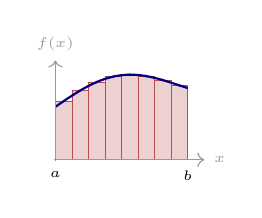
\begin{tikzpicture}[scale=0.42, font=\tiny]
    \foreach \i in {0,1,2,3,4,5,6,7} {
        \pgfmathsetmacro{\mx}{0.5*\i + 0.25}
        \pgfmathsetmacro{\hh}{1.6 + 0.6*sin(deg(\mx*0.85)) + 0.18*\mx}
        \draw[fill=harvardcrimson!18, draw=harvardcrimson!70, very thin]
            (0.5*\i, 0) rectangle (0.5*\i + 0.5, \hh);
        \fill[harvardcrimson] (\mx, \hh) circle (1.2pt);
    }
    \draw[thick, uzhblue, smooth, samples=80, domain=0:4]
        plot(\x, {1.6 + 0.6*sin(deg(\x*0.85)) + 0.18*\x});
    \draw[->, gray!80] (-0.05,0) -- (4.5,0) node[right, font=\tiny] {$x$};
    \draw[->, gray!80] (0,-0.05) -- (0,3.0) node[above, font=\tiny] {$f(x)$};
    \node[below, font=\tiny] at (0,-0.05) {$a$};
    \node[below, font=\tiny] at (4,-0.05) {$b$};
\end{tikzpicture}
\end{center}
\vspace{-0.6em}
{\tiny
With $\Delta x = (b-a)/N$, $x_i = a + i\Delta x$, $I = \int_a^b\! f(x)\,dx \approx \sum_i w_i\, f(x_i)$:
\vspace{-0.3em}
\begin{itemize}\itemsep0pt\setlength{\leftmargini}{1em}
    \item \emphc{Midpoint:} $I_N^{\text{mid}} = \Delta x \sum_{i=1}^N f(x_i^{\text{mid}})$, $\mathcal{O}(N^{-2})$
    \item \emphc{Trapezoid:} $I_N^{\text{trap}} = \tfrac{\Delta x}{2}\bigl[f(x_0) + 2\!\sum_{i=1}^{N-1}\!f(x_i) + f(x_N)\bigr]$, $\mathcal{O}(N^{-2})$
    \item \emphc{Simpson:} parabolic arcs through triples, $\mathcal{O}(N^{-4})$
    \item \emphc{Gauss--Hermite:} optimal nodes/weights for $e^{-x^2}$, $\mathcal{O}(N^{-(2Q-1)})$
\end{itemize}
}
{\tiny $d$-dim Cartesian grid: cost $\mathcal{O}(N^d)$, \emphc{curse of dimensionality}.}

\column{0.42\textwidth}
\begin{center}
{\scriptsize\textbf{Random: throw darts to estimate $\pi$}}\\[1pt]
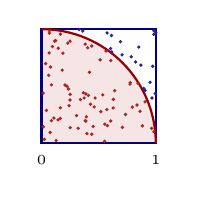
\begin{tikzpicture}[scale=1.45, font=\tiny]
    \fill[harvardcrimson!10] (0,0) -- (1,0) arc(0:90:1) -- cycle;
    \draw[thick, uzhblue] (0,0) rectangle (1,1);
    \draw[thick, harvardcrimson] (1,0) arc (0:90:1);
    \pgfmathsetseed{42}
    \foreach \i in {1,...,100} {
        \pgfmathsetmacro{\xx}{rnd}
        \pgfmathsetmacro{\yy}{rnd}
        \pgfmathsetmacro{\rsq}{\xx*\xx + \yy*\yy}
        \pgfmathparse{\rsq < 1 ? 1 : 0}
        \edef\inside{\pgfmathresult}
        \ifnum\inside=1
          \fill[harvardcrimson!85] (\xx,\yy) circle (0.016);
        \else
          \fill[uzhblue!85] (\xx,\yy) circle (0.016);
        \fi
    }
    \node[below, font=\tiny] at (0,-0.02) {$0$};
    \node[below, font=\tiny] at (1,-0.02) {$1$};
\end{tikzpicture}
\end{center}
\vspace{-0.4em}
{\tiny
Throw $N$ uniform darts at $\Omega = [0,1]^2$:
\[
\frac{\pi}{4} \;=\; \!\!\int_0^1\!\!\!\int_0^1\!\! \mathbf{1}[x^2+y^2 \le 1]\,dx\,dy \;\approx\; \frac{N_{\mathrm{in}}}{N}
\]
\vspace{-1.2em}
\[
\widehat{\pi}_N = 4 N_{\mathrm{in}}/N, \quad \text{error } \mathcal{O}(N^{-1/2})
\]
\emphc{Independent of dimension}, but slow.
}
\end{columns}
\end{frame}

% --- Slide 30: Gauss-Hermite quadrature ---
\begin{frame}{Quadrature, I: Gauss--Hermite}
\footnotesize
\textbf{Setup.} Generic shock dimension $d$, with $\bm\varepsilon' \sim \mathcal{N}(0, I_d)$.  Brock--Mirman has $d=1$ (one productivity shock); the IRBC chapter will use $d=N+1$ ($N$ country shocks plus one aggregate).  We develop the framework here so it is ready for both cases.

\vspace{0.3em}
\textbf{One dimension.} Gauss--Hermite uses $Q$ nodes $\{\varepsilon_q\}$ (Hermite-polynomial roots) and weights $\{w_q\}$:
\[
\E{h(\varepsilon)} \;=\; \int_{-\infty}^{\infty} h(\varepsilon)\,\frac{e^{-\varepsilon^2/2}}{\sqrt{2\pi}}\,d\varepsilon \;\approx\; \sum_{q=1}^{Q} w_q\, h(\varepsilon_q),
\]
\emph{exact} for univariate polynomials of degree $\le 2Q-1$.

\vspace{0.3em}
\textbf{Tensor product in $d$ dimensions.} Combine 1D rules along each axis:
\[
\E{h(\bm\varepsilon')} \;\approx\; \sum_{q_1=1}^{Q}\!\!\cdots\!\!\sum_{q_d=1}^{Q} \Bigl(\textstyle\prod_{j} w_{q_j}\Bigr)\, h(\varepsilon_{q_1}, \ldots, \varepsilon_{q_d}).
\]
\vspace{-0.4em}
\begin{itemize}\itemsep1pt
    \item \emphc{Strength:} polynomial-exact in each coordinate, very accurate at low $d$.  For $d=1$ (Brock--Mirman) a $Q=3$ rule is essentially exact.
    \item \emphc{Weakness:} cost $Q^{d}$ blows up exponentially. For $Q=3$, $d=11$ (IRBC, $N=10$): $\sim 1.8\times 10^5$ nodes per state.
\end{itemize}
\end{frame}

% --- Slide 30: Monomial / Stroud-3 ---
\begin{frame}{Quadrature, II: Monomial (Stroud-3) Rule}
\footnotesize
\textbf{Idea.} Drop full polynomial-exactness in every coordinate, keep exactness for total degree $\le 3$. Place nodes only on the principal axes of the $d$-dimensional shock space:
\[
\boxed{\;
\E{h(\bm\varepsilon')} \;\approx\; \frac{1}{2d} \sum_{k=1}^{d} \Bigl[\, h\bigl(+\sqrt{d}\,\bm{e}_k\bigr) + h\bigl(-\sqrt{d}\,\bm{e}_k\bigr)\Bigr]
\;}
\]
where $\bm{e}_k$ is the $k$-th standard basis vector, giving $2d$ nodes at common radius $\sqrt{d}$.  For Brock--Mirman ($d=1$) this reduces to two nodes at $\pm 1$ (exact for univariate polynomials of degree $\le 3$); for IRBC ($d=N+1$) it gives $2(N+1)$ nodes.

\vspace{0.5em}
\begin{columns}[T]
\column{0.52\textwidth}
\textbf{What it integrates exactly}
\begin{itemize}\itemsep1pt
    \item $\mathbb{E}[\varepsilon_i'] = \mathbb{E}[\varepsilon_i'^{\,3}] = 0$ ($\pm$-symmetry).
    \item $\mathbb{E}[\varepsilon_i' \varepsilon_j'] = 0$, $i \neq j$ (each node lies on one axis).
    \item $\mathbb{E}[\varepsilon_i'^{\,2}] = 1$ (variance preserved).
\end{itemize}
\textbf{Where it stops}
\begin{itemize}\itemsep1pt
    \item $\mathbb{E}[\varepsilon_i'^{\,4}]$ gives $d$ vs.\ truth $3$, a controlled fourth-order bias.
\end{itemize}

\column{0.46\textwidth}
\begin{block}{Why DEQNs love it}
\scriptsize
The integrand $h(\bm\varepsilon')$ is the policy network composed with model primitives, smooth and only mildly nonlinear. Degree-3 exactness is enough for Euler-error tolerances of $\sim\!10^{-3}$ on IRBC-class problems.\\[2pt]
\emphc{(Pichler 2011; Maliar \& Maliar 2014)}
\end{block}
\end{columns}
\end{frame}

% --- Slide 31: Cost comparison ---
\begin{frame}{Quadrature, III: Cost and Rules of Thumb}
\footnotesize
\textbf{Per-state quadrature cost} ($Q=3$ for the tensor-product rule):
\vspace{0.2em}
\begin{center}
\renewcommand{\arraystretch}{1.05}
\begin{tabular}{@{}rrrrl@{}}
\toprule
$N$ & shocks $N{+}1$ & tensor product $3^{N+1}$ & monomial $2(N{+}1)$ & speed-up\\
\midrule
$2$  & $3$  & $27$           & $6$   & $\sim\! 5\times$\\
$5$  & $6$  & $729$          & $12$  & $\sim\! 60\times$\\
$10$ & $11$ & $177{,}147$    & $22$  & $\sim\! 8{,}000\times$\\
$20$ & $21$ & $\sim\! 10^{10}$ & $42$  & $\sim\! 2\!\times\!10^8\times$\\
\bottomrule
\end{tabular}
\end{center}

\vspace{0.4em}
\begin{columns}[T]
\column{0.49\textwidth}
\begin{block}{Default rules of thumb}
\scriptsize
\begin{itemize}\itemsep1pt
    \item $N{+}1 \le 4$: tensor-product GH, $Q\!=\!5$.
    \item $5 \le N{+}1 \lesssim 30$: Stroud-3 monomial.
    \item $N{+}1 \gtrsim 30$ or fat-tailed integrands: QMC (Sobol $+$ inverse-CDF).
\end{itemize}
\end{block}

\column{0.49\textwidth}
\begin{block}{Practical notes}
\scriptsize
\begin{itemize}\itemsep1pt
    \item Only the quadrature \emphc{kernel} changes; same DEQN loss, same training loop.
    \item Validate by tightening the rule and checking the Euler-error histogram is stable.
    \item Full derivations: lecture script $\S 3.5$.
\end{itemize}
\end{block}
\end{columns}
\end{frame}

% --- Slide 32: Diagnostics ---
\begin{frame}{Diagnostics: How Do We Know Training Worked?}
\footnotesize
\textbf{Never trust a loss curve alone.}  On an independent \emph{test} simulation of the trained policy, run these four complementary checks:

\vspace{0.3em}
\begin{enumerate}\itemsep2pt
    \item \emphc{Euler-error distribution.}  Histogram $\log_{10}|e_{\mathrm{REE}}|$ on train and test states; both should peak near $10^{-3}$ or below, with no fatter right tail on test.
    \item \emphc{Policy-function benchmark.}  Overlay the DEQN policy on the analytic $s^\star=\beta\alpha$ for Brock--Mirman; for richer models, on a trusted reference (time iteration, perturbation).
    \item \emphc{Ergodic-set coverage.}  Scatter test states in the $(K_t,\log z_t)$ plane; the cloud should trace the training ergodic set~---~not collapse to a point, not spread like a grid.
    \item \emphc{Sanity checks.}  Verify accounting identities (budget, market clearing, non-negativity); check that ergodic moments (mean $K$, $\mathrm{std}(z)$, autocorrelations) match analytic or pre-computed values.
\end{enumerate}

\vspace{0.3em}
\begin{center}
{\scriptsize \emphc{Green flags:} low Euler error, matches benchmark, ergodic coverage, identities hold.\ \ \emphc{Red flags:} NaNs, fat tails, clamped policy, violated identities.}
\end{center}

\vspace{0.1em}
{\scriptsize When no closed-form benchmark exists, draw inspiration from the \emphc{VVUQ literature}~---~Verification, Validation \& Uncertainty Quantification (Roache 1998; Oberkampf \& Roy 2010; ASME V\&V 10/20)~---~which formalises residual convergence, solution verification, and error-bound reporting for computational models.}
\end{frame}

% --- Slide: Loss-kernel choice (Brock-Mirman) -------------------------------
\begin{frame}{Choice of Training Loss: Six Kernels}
\footnotesize
The loss kernel is a \emphc{modeling decision}, not a default.  Same Euler residual $r$, same network, same data, only the reduction $r\!\mapsto\!\ell$ changes:

\vspace{0.4em}
\begin{center}
\renewcommand{\arraystretch}{1.15}
\setlength{\tabcolsep}{4pt}
\begin{tabular}{@{}lll@{}}
\toprule
\textbf{Kernel} & \textbf{Formula} & \textbf{Character} \\
\midrule
MSE      & $\tfrac1B\sum r^2$                                & quadratic; canonical default \\
MAE      & $\tfrac1B\sum |r|$                                 & constant gradient $\Rightarrow$ \emphc{stalls at small $|r|$} \\
Huber    & quad.\ for $|r|\!\le\!\delta$, linear above       & robust hybrid, but \emphc{kink at $|r|{=}\delta$} \\
Quantile & pinball at $\tau{=}0.9$                            & trains the upper $\tau$-quantile only \\
CVaR     & mean of top $10\%$ of $|r|$                        & explicitly trains the worst-case states \\
\textbf{LogCosh} & $\tfrac1B\sum\log\cosh(r)$                   & $C^\infty$: $\tfrac12 r^2$ near $0$, $|r|{-}\log 2$ in tails, \emphc{no kink} \\
\bottomrule
\end{tabular}
\end{center}

\vspace{0.6em}
{\scriptsize Same Brock--Mirman model, full depreciation so $s^\star = \alpha\beta$ is in closed form; same network (2$\times$32 swish, sigmoid head); same Adam optimizer; same CRN training stream.  Six runs differ \emph{only} in the reduction applied to the residual vector.}
\end{frame}

\begin{frame}{Loss Kernels: Convergence on Brock--Mirman}
\begin{center}

\includegraphics[width=0.98\linewidth]{figures/loss_kernel_convergence.png}
\end{center}

\vspace{0.2em}
{\footnotesize Mean / $p_{90}$ / $p_{99}$ of the absolute relative Euler error $|r|$ on a fixed evaluation grid, vs.\ training episode (log scale, 5000 episodes per kernel).  \emphc{LogCosh and MSE} reach the lowest mean residual.  \emphc{Huber and CVaR} produce the narrowest tail.  \emphc{MAE stalls} at a noise floor.}
\end{frame}

\begin{frame}{Loss-Kernel Comparison: What to Take Away}
\scriptsize
\begin{itemize}\itemsep1.5pt
    \item \emphc{LogCosh converges most smoothly:} the only $C^\infty$ kernel that is MSE-like near $r=0$ \emph{and} MAE-like in the tails, no kink anywhere.  Lowest-risk default when the residual distribution is unknown.
    \item \emphc{MAE stalls} at a noise floor: constant gradient magnitude prevents smaller steps as residuals shrink.
    \item \emphc{Huber is robust} but its kink at $|r|{=}\delta$ can introduce small oscillations.
    \item \emphc{Quantile and CVaR} narrow $p_{99}$ at the cost of mean residual.  Use them when worst-case policy quality matters (binding constraints, rare-but-consequential states, regulatory back-tests).
    \item \emphc{Evaluate on the economic metric}~---~Euler error along simulated paths, in CE-welfare-loss units~---~not on the training loss itself.  The CE ranking is generally not the training-loss ranking.
\end{itemize}

\vspace{0.4em}
\begin{exampleblock}{Practical default}
\textbf{MSE} remains the canonical default, but \textbf{LogCosh} is a smooth, kink-free alternative that should be benchmarked alongside it before defaulting; \textbf{Huber / Quantile / CVaR} when the worst-case state matters.
\end{exampleblock}

\vspace{0.2em}
{\scriptsize Companion notebook: \texttt{lectures/lecture\_03\_deep\_equilibrium\_nets/code/lecture\_03\_05\_StochasticBM\_LossComparison.ipynb}.}
\end{frame}

% ============================================================================
% PART IV: PARALLELIZATION AND HPC
% ============================================================================

% --- Slide 26: Part IV Divider ---
\begin{frame}{}
\vfill
\begin{center}
{\Huge \textcolor{uzhblue}{\textbf{Part IV}}}\\[12pt]
{\LARGE Parallelization \& HPC}
\end{center}
\vfill
\end{frame}

% --- Slide 27: HPC Quote ---
\begin{frame}{}
\vfill
\begin{center}
{\Large\itshape
``To pull a bigger wagon, it is easier to add more oxen\\
than to grow a gigantic ox.''}

\vspace{0.8cm}
{\normalsize --- Gropp, Lusk \& Skjellum (1999)}\\[4pt]
{\small\itshape Using MPI: Portable Parallel Programming}
\end{center}
\vfill
\end{frame}

% --- Slide 28: Data Parallelism ---
\begin{frame}{Data Parallelism for DEQNs}
\textbf{Idea:} distribute training data across \emphc{multiple workers} (GPUs/CPUs).

\vspace{0.4em}
\begin{center}
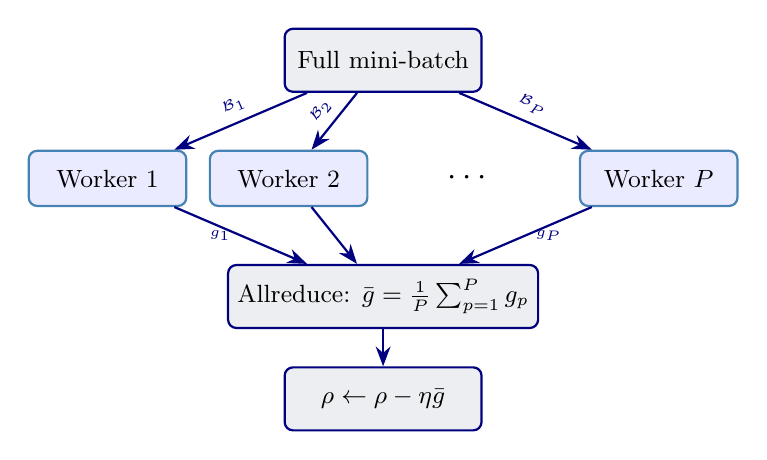
\begin{tikzpicture}[
    mlstep/.style={rectangle, draw=uzhblue, thick, fill=uzhgreylight,
        minimum width=2.5cm, minimum height=0.8cm, font=\small,
        rounded corners=3pt},
    worker/.style={rectangle, draw=softblue, thick, fill=blue!8,
        minimum width=2.0cm, minimum height=0.7cm, font=\small,
        rounded corners=3pt},
    arr/.style={-{Stealth[length=2.5mm]}, thick, uzhblue}
]
    \node[mlstep] (data) at (0,0) {Full mini-batch};
    \node[worker] (w1) at (-3.5,-1.5) {Worker 1};
    \node[worker] (w2) at (-1.2,-1.5) {Worker 2};
    \node[font=\large] (dots) at (1.1,-1.5) {$\cdots$};
    \node[worker] (wP) at (3.5,-1.5) {Worker $P$};

    \node[mlstep] (grad) at (0,-3.0) {Allreduce: $\bar{g} = \frac{1}{P}\sum_{p=1}^P g_p$};
    \node[mlstep] (upd) at (0,-4.3) {$\rho \leftarrow \rho - \eta \bar{g}$};

    \draw[arr] (data) -- (w1) node[midway, above, font=\tiny, sloped] {$\mathcal{B}_1$};
    \draw[arr] (data) -- (w2) node[midway, above, font=\tiny, sloped] {$\mathcal{B}_2$};
    \draw[arr] (data) -- (wP) node[midway, above, font=\tiny, sloped] {$\mathcal{B}_P$};

    \draw[arr] (w1) -- (grad) node[midway, left, font=\tiny] {$g_1$};
    \draw[arr] (w2) -- (grad);
    \draw[arr] (wP) -- (grad) node[midway, right, font=\tiny] {$g_P$};

    \draw[arr] (grad) -- (upd);
\end{tikzpicture}
\end{center}

\vspace{0.2em}
{\small Implemented via \textbf{Horovod}/MPI. Each worker computes a local gradient; \emphc{allreduce} averages them.}
\end{frame}

% --- Slide 29: Parallelization Scheme ---
\begin{frame}{DEQN Parallelization Scheme}
\begin{center}
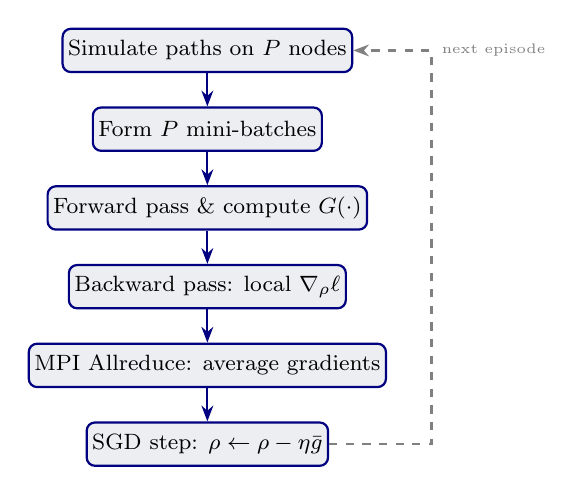
\begin{tikzpicture}[
    mlstep/.style={rectangle, draw=uzhblue, thick, fill=uzhgreylight,
        minimum width=2.8cm, minimum height=0.55cm, font=\footnotesize,
        rounded corners=3pt, inner sep=2pt},
    arr/.style={-{Stealth[length=2mm]}, thick, uzhblue}
]
    \node[mlstep] (sim) at (0,0) {Simulate paths on $P$ nodes};
    \node[mlstep] (mb) at (0,-1.0) {Form $P$ mini-batches};
    \node[mlstep] (fwd) at (0,-2.0) {Forward pass \& compute $G(\cdot)$};
    \node[mlstep] (bwd) at (0,-3.0) {Backward pass: local $\nabla_\rho \ell$};
    \node[mlstep] (all) at (0,-4.0) {MPI Allreduce: average gradients};
    \node[mlstep] (step) at (0,-5.0) {SGD step: $\rho \leftarrow \rho - \eta \bar{g}$};

    \draw[arr] (sim) -- (mb);
    \draw[arr] (mb) -- (fwd);
    \draw[arr] (fwd) -- (bwd);
    \draw[arr] (bwd) -- (all);
    \draw[arr] (all) -- (step);

    \draw[arr, dashed, gray] (step.east) -- ++(1.3,0) |- (sim.east)
        node[midway, right, font=\tiny, text=gray] {next episode};
\end{tikzpicture}
\end{center}

{\small Communication cost $\sim \mathcal{O}(|\rho|)$ per step, independent of data size.}
\end{frame}

% --- Slide 30: Scalability ---
\begin{frame}{Illustrative Scaling Pattern (Schematic)}
\begin{center}
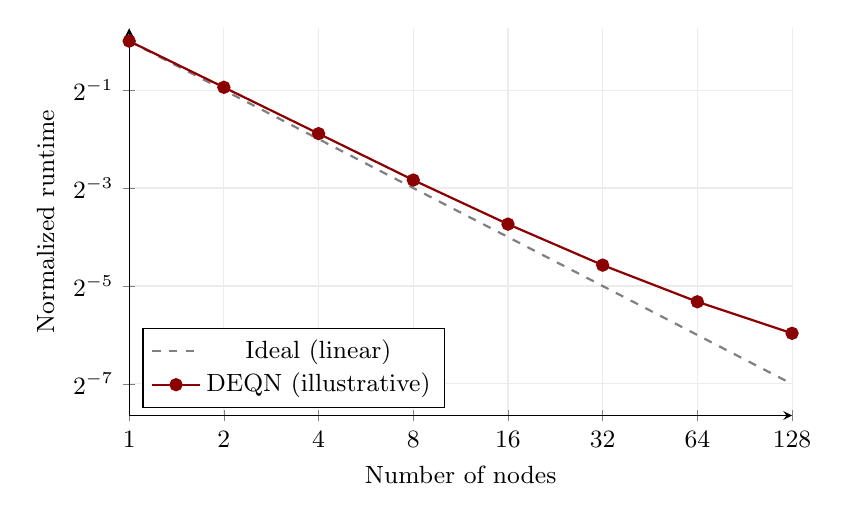
\begin{tikzpicture}
\begin{axis}[
    width=10cm, height=6.5cm,
    xlabel={Number of nodes},
    ylabel={Normalized runtime},
    xlabel style={font=\small},
    ylabel style={font=\small},
    tick label style={font=\small},
    xmode=log, ymode=log,
    log basis x=2, log basis y=2,
    xmin=1, xmax=128, ymin=0.005, ymax=1.2,
    grid=major, grid style={gray!15},
    legend style={font=\small, at={(0.02,0.02)}, anchor=south west},
    axis lines=left,
    xtick={1,2,4,8,16,32,64,128},
    xticklabels={1,2,4,8,16,32,64,128},
]
    % Ideal scaling
    \addplot[thick, dashed, gray, domain=1:128, samples=8]
        {1/x};
    \addlegendentry{Ideal (linear)}

    % Realized scaling (slightly worse)
    \addplot[thick, darkred, mark=*, mark size=2pt]
        coordinates {
            (1, 1.0) (2, 0.52) (4, 0.27) (8, 0.14)
            (16, 0.075) (32, 0.042) (64, 0.025) (128, 0.016)
        };
    \addlegendentry{DEQN (illustrative)}
\end{axis}
\end{tikzpicture}
\end{center}

{\small Schematic message only: synchronous data parallelism is often close to linear for moderate worker counts; large clusters become increasingly communication-limited.}
\end{frame}

% --- Slide 31a: Preview of the exercises (KKT/FB) ---
\begin{frame}{Preview: the Morning Exercises}
\footnotesize
\textbf{Exercises 03/04 extend Brock--Mirman in two directions:}
\begin{enumerate}\itemsep2pt
    \item \emph{Endogenous labor} with a non-negativity constraint on leisure, introducing a \emph{Karush--Kuhn--Tucker} multiplier $\mu_t \ge 0$.
    \item A \emph{6-period OLG} economy with a borrowing constraint on the young, again KKT with $\mu_t \ge 0$.
\end{enumerate}

\vspace{0.4em}
\textbf{Why this matters for DEQNs.}  A KKT system imposes complementary slackness $\mu \ge 0,\ g \ge 0,\ \mu\,g = 0$.  This cannot be encoded as a smooth equation, so we replace it by the \emph{Fischer--Burmeister} function
\[
\phi_{\mathrm{FB}}(a,b) \;=\; a + b - \sqrt{a^2 + b^2}, \qquad \phi_{\mathrm{FB}}(a,b) = 0 \ \Longleftrightarrow\ a \ge 0,\ b \ge 0,\ a\,b = 0,
\]
which is smooth everywhere except at the origin and is fully differentiable by autodiff.

\vspace{0.3em}
{\footnotesize \emphc{Exercise loss.}  The notebooks sum a squared \emph{Euler} residual and a squared \emph{FB} residual for each constraint; both are minimized jointly.  Details: see the IRBC chapter of the lecture script (KKT sub-section).}
\end{frame}

% --- Slide 31: Hands-on Notebooks (wrap-up) ---
\begin{frame}{Hands-on Notebooks}
\textbf{Four notebooks} accompany this lecture:

\vspace{0.4em}
\begin{enumerate}\itemsep2pt
    \item \texttt{01\_Brock\_Mirman\_1972\_DEQN.ipynb}\\
    {\small Deterministic Brock--Mirman, \emphc{exogenous uniform sampling} of states.}

    \item \texttt{02\_Brock\_Mirman\_Uncertainty\_DEQN.ipynb}\\
    {\small Stochastic Brock--Mirman ($\varrho > 0$, $\sigma_z > 0$), \emphc{simulation-based sampling} on the ergodic set.}

    \item \texttt{03\_DEQN\_Exercises\_Blanks.ipynb} (exercises, blank template for student populate)

    \item \texttt{04\_DEQN\_Exercises\_Solutions.ipynb} (exercises, solved)
\end{enumerate}

\vspace{0.3em}
{\footnotesize Notebooks 01--02 illustrate the sampling progression: uniform random $\to$ simulated trajectories.  Notebooks 03--04 add KKT multipliers + Fischer--Burmeister + the 6-period OLG structure previewed on the previous slide.}

\vspace{0.4em}
All notebooks are in the course repository.
\end{frame}

% --- Questions ---
\begin{frame}{}
\begin{columns}[c]
\column{0.45\textwidth}
\begin{center}
{\Huge \textcolor{uzhblue}{\textbf{Questions?}}}

\vspace{1.0cm}
{\large Simon Scheidegger}\\[4pt]
{\small HEC, University of Lausanne}\\[4pt]
\url{https://sischei.github.io}

\vspace{0.6cm}
{\small Materials:~~\url{https://github.com/sischei/Deep_Learning_for_Solving_And_Estimating_Dynamic_Economic_Models}}
\end{center}

\column{0.45\textwidth}
\begin{center}
\textbf{Next up:}\\[6pt]
{\large DEQN Exercises}\\[12pt]
\end{center}
\end{columns}
\end{frame}

\end{document}
